% BUBBLE-BLUE, NetMob 2026 two-page extended abstract.
% Layout follows the official NetMob Word template (Optica length-check):
% US Letter, two columns, 10 pt body. For submission, paste the title,
% authors, body and bibliography into the official NetMob Overleaf template.
% Page 1: idea, state of the art, start of the design.
% Page 2: left column ends the design, right column holds the results.
% Compiler: pdfLaTeX, then BibTeX, then pdfLaTeX twice.
\documentclass[10pt,twocolumn,letterpaper]{article}
\usepackage[letterpaper,left=17.5mm,right=17.5mm,top=19mm,bottom=22mm,columnsep=7.9mm]{geometry}
\usepackage[T1]{fontenc}
\usepackage[utf8]{inputenc}
\usepackage{mathptmx}
\usepackage[scaled=0.92]{helvet}
\usepackage{amsmath}
\usepackage{booktabs}
\usepackage{url}
\usepackage[hidelinks]{hyperref}
\usepackage{tikz}
\usetikzlibrary{positioning,calc}
\usepackage[font={footnotesize,sf},labelfont=bf,labelsep=period,skip=3pt]{caption}
\usepackage{titlesec}
\usepackage{authblk}
\usepackage{enumitem}
\usepackage{cite}

\titleformat{\section}{\sffamily\bfseries\normalsize\MakeUppercase}{\thesection.}{0.5em}{}
\titlespacing*{\section}{0pt}{5pt}{2pt}
\newcommand{\sub}[1]{\smallskip\noindent\textsf{\textbf{#1}}\enspace}
\renewcommand{\Authfont}{\sffamily\large}
\renewcommand{\Affilfont}{\sffamily\footnotesize}
\setlength{\affilsep}{2pt}
\setlist{nosep, leftmargin=*}
\pagestyle{empty}
\hyphenation{Blue-tooth BUBBLE-BLUE}

\title{\vspace{-6mm}\sffamily\bfseries\LARGE BUBBLE-BLUE: private group messaging\\
over an open Bluetooth mesh, measured on six boards}
\author[1]{Paul-Maxence Baraton}
\author[1]{Nadjib Achir}
\author[1]{Philippe Jacquet}
\author[2]{Wilfred Doré}
\affil[1]{Inria, France; \texttt{\{paul-maxence.baraton, nadjib.achir, philippe.jacquet\}@inria.fr}}
\affil[2]{Qualcomm, France; \texttt{wdore@qti.qualcomm.com}}
\date{\vspace{-8mm}}

\begin{document}
\maketitle
\thispagestyle{empty}

\noindent\textsf{\textbf{Abstract.}} \textsf{BUBBLE-BLUE is a multi-hop
private group that rides on an open Bluetooth Low Energy (BLE) mesh: any
node may relay, only key holders may read. We present its design and the
first implementation, over BLE L2CAP connection-oriented channels and
without pairing, on six single-board computers. Spread through a building
on battery, the boards formed a four-hop line of about 60\,m on their
own, with a median delay of 162\,ms at the far end.}

\section{The idea}

Local communication without infrastructure still collapses onto a Wi-Fi
access point or a phone operating system that will not host a
third-party mesh. Yet the settings that need it most are those where
infrastructure is absent, saturated or distrusted: a crowd at an event, a
site without coverage, an emergency response. Bluetooth is on every
device and needs no operator.

BUBBLE-BLUE~\cite{achir2025bb} separates two things that existing
Bluetooth meshes merge. The \emph{topological mesh} is open: any node may
join it and relay traffic, including traffic it cannot read. The
\emph{bubbles} are private: a group exists only for the holders of its
key. A stranger's phone can therefore extend the reach of a conversation
it will never see. To keep the cost of flooding low, only an elected
backbone, a connected dominating set (CDS), retransmits. The original
note gave the algorithms and simulations. This work contributes the BLE
transport and frame format, a revocation protocol that reaches members
several hops away, and measurements on real boards, in a room and across
a building.

\section{State of the art}

\sub{Bluetooth meshes and messengers.} The SIG Mesh
profile~\cite{mesh-profile} is a managed-flooding stack for lighting and
sensors; nodes are provisioned, and a relay must hold the network key.
BitChat~\cite{bitchat} shows that a BLE-only chat can reach consumer
scale; it floods over GATT without a backbone. Bridgefy
flooded messages among protesters, and its cryptanalysis~\cite{albrecht2021}
shows what a mesh used in a crowd must withstand: impersonation, tracking
and denial of service.
Briar~\cite{briar} synchronises between \emph{pre-paired} contacts over
Classic Bluetooth, Wi-Fi and Tor. Reticulum~\cite{reticulum} routes to
cryptographic identities over any link.

\sub{Backbones for broadcast.} Electing a subset of forwarders is classic
in ad hoc networks: Wu and Li's marking rule~\cite{wuli1999} yields a CDS
from two-hop knowledge, and multipoint relays~\cite{qayyum2002}, the basis
of OLSR, reduce flooding from each node's view. BLE makes
this matter more than Wi-Fi, because it has no native broadcast on a
connection: every local flood is a sequence of unicasts.

\sub{The gap.} Table~\ref{tab:not} places BUBBLE-BLUE: none of the other
systems lets a node sit in an elected backbone and relay for a group it
does not belong to.

\begin{table}[t]
\centering
\caption{Where BUBBLE-BLUE sits. ``Open relay'': a node may forward a
frame it cannot decrypt.}
\label{tab:not}
\footnotesize
\begin{tabular}{@{}lccc@{}}
\toprule
System & Data plane & Backbone & Open relay \\
\midrule
SIG Mesh~\cite{mesh-profile} & managed flood & provisioned & no \\
BitChat~\cite{bitchat} & GATT flood & none & n/a \\
Briar~\cite{briar} & RFCOMM, Wi-Fi, Tor & contacts & no \\
Reticulum~\cite{reticulum} & multi-transport & identities & no \\
BUBBLE-BLUE & LE CoC & elected CDS & yes \\
\bottomrule
\end{tabular}
\end{table}

\section{Design}

\sub{Links without pairing.} A node advertises a compact presence record
in a connectable BLE advertisement: an anonymous identifier, a relay
flag, and the address at which it accepts connections (manufacturer data
under company identifier \texttt{0xFFFF}, reserved by the Bluetooth SIG
for testing, marking the prototype as experimental). Neighbours then open
an L2CAP connection-oriented channel at security level \emph{low}: no
pairing, no bond, no allow-list. Membership is a 32-byte group key, not a
Bluetooth relationship. Periodic HELLO messages fill a neighbour table; a
neighbour silent for three periods (15\,s) is dropped.

\sub{One frame, two planes.} Every frame starts with a 26-byte clear
header: type, source, destination, TTL, sequence and timestamp. The
payload is sealed with AES-256-GCM under a per-packet key,
HKDF-SHA256 of the group key with source, sequence and timestamp. All
header fields but TTL are authenticated. A relay that does not hold the
key can thus decrement TTL and forward the frame; it cannot read the text
or forge its sender. A message of up to 470 bytes fits one frame.

\sub{Who relays.} Each node applies the Wu--Li rule~\cite{wuli1999} to
its two-hop view and relays if it is marked, or if it bridges two links
the backbone has not covered. Duplicates are suppressed on (source,
sequence), so a flood crosses each relay once. The receiving screen
shows the hop count and the neighbour a message came through.

\sub{Removing a member.} The coordinator, the member with the smallest
anonymous identifier, revokes by rotating the group key and flooding it
wrapped under pairwise X25519 keys, skipping the victim. The victim keeps
relaying but can no longer read. Keys of members beyond one hop arrive
by a signed ANNOUNCE every 30\,s; revoking before then is refused, which
defines a join window.

\sub{What an adversary can do.} A passive radio in range learns who
transmits, toward which address, and how far a frame may still go; it
does not learn the text. The Bluetooth address is stable and in clear,
because that is how a neighbour is redialled without a bond: payload
privacy is not location privacy. An active non-member can make the
backbone carry junk, reset TTL, which is not authenticated, or pre-empt
a (source, sequence) pair at a relay to cause selective loss. A member
who controls its address can grind it to become coordinator. These are
accepted limits of the prototype.

\sub{On real boards.} A privileged daemon owns the Bluetooth adapter;
touch screens are unprivileged clients. Screens are three Thundercomm
RUBIK Pi~3 (Qualcomm QCS6490, Ubuntu 24.04, kernel 6.8, BlueZ 5.72);
relays are three Arduino UNO~Q (Qualcomm QRB2210, Debian 13, kernel 7.0,
BlueZ 5.82). On the tested UNO~Q image the controller cannot dial while
it is peripheral on any link, so relays always dial and screens never do:
every path alternates screen and relay, and on a table the graph is
$K_{3,3}$ (Fig.~\ref{fig:stand}). The same kernel leaks one L2CAP
signalling identifier per received credit, so links are recycled before
the pool of 254 runs out, and a controller that stops answering is
reloaded locally without rebooting the board.

\begin{figure}[t]
\centering
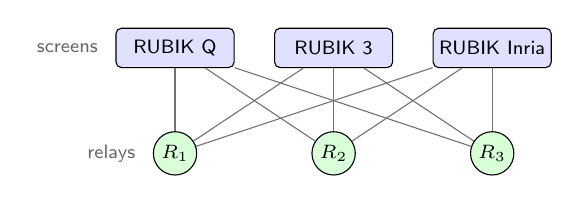
\begin{tikzpicture}[font=\scriptsize\sffamily,
  s/.style={draw, rounded corners=2pt, fill=blue!12, minimum width=15mm, minimum height=5mm, inner sep=1pt},
  r/.style={draw, circle, fill=green!15, minimum size=5.5mm, inner sep=0pt}]
  \node[s] (a) {RUBIK Q};
  \node[s, right=5mm of a] (b) {RUBIK 3};
  \node[s, right=5mm of b] (c) {RUBIK Inria};
  \node[r, below=8mm of a] (r1) {$R_1$};
  \node[r, below=8mm of b] (r2) {$R_2$};
  \node[r, below=8mm of c] (r3) {$R_3$};
  \foreach \x in {a,b,c} \foreach \y in {r1,r2,r3} \draw[black!55] (\x)--(\y);
  \node[left=1mm of a, text=black!60] {screens};
  \node[left=1mm of r1, text=black!60] {relays};
\end{tikzpicture}
\caption{The demonstration stand: every message between two screens
crosses one of three relays.}
\label{fig:stand}
\end{figure}

\newpage
\section{Results}

\begin{table}[t]
\centering
\caption{Measurements on the six boards.}
\label{tab:res}
\footnotesize
\begin{tabular}{@{}p{0.70\columnwidth}r@{}}
\toprule
\multicolumn{2}{@{}l}{Stand ($K_{3,3}$, one room)} \\
\midrule
Messages received by the five other boards & 75/75 \\
Rebooted screen reads the group, after daemon start & 4.4\,s \\
Relay whose controller was cut reads again, no reboot & 130\,s \\
Revoked board reads the next message (2 trials) & no \\
\midrule
\multicolumn{2}{@{}l}{Four-hop line (building, battery, $\sim$15\,m spacing)} \\
\midrule
Messages received four hops away & 76/79 \\
Median delay, 1 / 2 / 3 / 4 hops (ms) & 85 / 101 / 143 / 162 \\
Last link carried away: held to & $\sim$30\,m \\
\bottomrule
\end{tabular}
\end{table}

\begin{figure}[t]
\centering
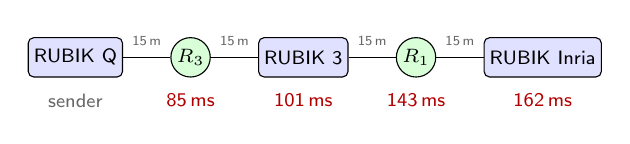
\begin{tikzpicture}[font=\scriptsize\sffamily,
  s/.style={draw, rounded corners=2pt, fill=blue!12, minimum height=5mm, inner sep=2pt},
  r/.style={draw, circle, fill=green!15, minimum size=5mm, inner sep=0pt}]
  \node[s] (a) {RUBIK Q};
  \node[r, right=6mm of a] (b) {$R_3$};
  \node[s, right=6mm of b] (c) {RUBIK 3};
  \node[r, right=6mm of c] (d) {$R_1$};
  \node[s, right=6mm of d] (e) {RUBIK Inria};
  \foreach \u/\v in {a/b,b/c,c/d,d/e}{
    \draw (\u)--(\v);
    \node[above=0.2mm, font=\tiny\sffamily, text=black!60] at ($(\u.east)!0.5!(\v.west)$) {15\,m};}
  \foreach \x/\t in {b/85, c/101, d/143, e/162}
    \node[below=0.8mm of \x, text=red!70!black] {\t\,ms};
  \node[below=0.8mm of a, text=black!60] {sender};
\end{tikzpicture}
\caption{The line the boards formed on their own; median delays.}
\label{fig:line}
\end{figure}

\sub{On the stand.} Every message reached the five other boards
(Table~\ref{tab:res}). Joining is dominated by the boot: a rebooted
screen read the group 4.4\,s after its daemon started. AES-GCM (30k--173k packets/s) is
far above the link; the bottleneck is the relay's Bluetooth stack, near
10\,msg/s.

\sub{Across a building.} With the boards about 15\,m apart and one relay
off, the mesh formed a four-hop line by itself (Fig.~\ref{fig:line}).
From on-board logs (clocks within 50\,ms), the far end received 76 of 79
messages, missing only the three sent while the line formed; each hop
adds a few tens of milliseconds.
Carried away, the far screen's link held to about 30\,m, dropped, and
returned within seconds of the board coming back: mobility appears as
ordinary link churn. When the sender's only relay lost power, the line
was dark for 95\,s: a line has no detour.

\sub{In simulation and next.} On a unit-disk radio the backbone adds no
path stretch, and TTL~10 spans about twenty nodes (a simulation result).
A day-long battery run is under way; the link logs form a contact graph
on which to replay the protocol under real mobility traces.

\smallskip
\noindent\textsf{\textbf{Acknowledgment.}} Boards from the Qualcomm
University Platforms program. AI-assisted tools were used for software,
analysis and editing; the authors checked all results.

\scriptsize
\let\oldthebib\thebibliography
\renewcommand{\thebibliography}[1]{\oldthebib{#1}\setlength{\itemsep}{0pt}\setlength{\parsep}{0pt}}
\titlespacing*{\section}{0pt}{3pt}{1pt}
\bibliographystyle{IEEEtran}
\bibliography{refs}

\end{document}
